\documentclass{article}

\usepackage{hyperref}
\hypersetup{
	colorlinks=true,
	linkcolor=blue,
	filecolor=magenta,      
	urlcolor=cyan
}
\usepackage[american]{circuitikz}
\ctikzset{tripoles/mos style/arrows}
\ctikzset{transistors/arrow pos=end}
\ctikzset{label/align = straight}
\usepackage{siunitx}
\usepackage{amsmath}

\begin{document}
	This document describes how electrons move and answers some questions about intrinsic silicon and doped silicon
	\section{From Bohr model to +/- charges in a material}
		When we evaluate methods and electronic components, we often think about +/- charges flowing in a material, like the image below
		\begin{center}
			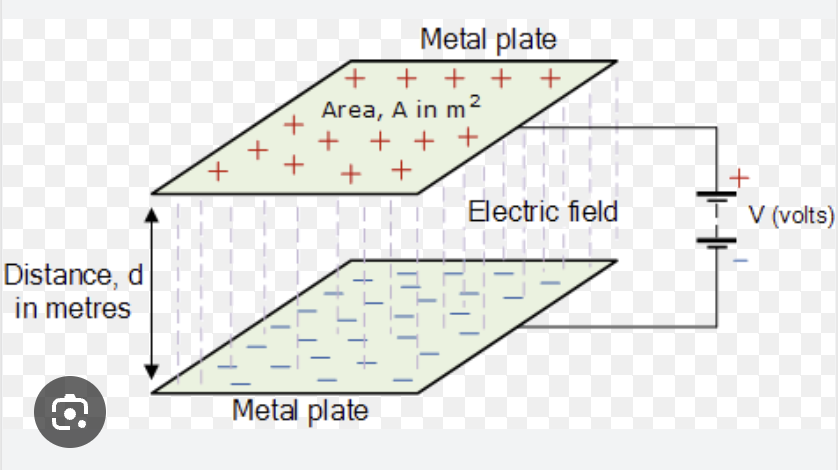
\includegraphics[width=\textwidth]{img/capacitor.png}
		\end{center}
		but how does that relate to a bohr model? More specifically, how does electrons / holes in a bohr model be to move across atoms?\\
		we know that there are energy bands, in a bohr model, every material has a certain number of valence electrons in its \textbf{valence shell}. Silicon has 4, Boron has 3, etc. In order for those electrons move freely, it needs a certain amount of energy in order for it to jump across the forbidden gap and into the conduction band.\\
		Note that the valence shell not the same as the \textbf{valence bands}. 
		Electrons in each shell (orbital) has a certain range of energy. Now looking at the electrons in the valence shell. Normally they have the level of energy in the range of \textbf{the valence band}, but when they are excited and gain energy, they can jump across the forbidden gap and into the \textbf{conduction band}. That's when they jump out of the valence shell (orbital) and become free electrons. \\
		In other words, the orbitals in the bohr model are sort of related to energy. Electrons in the outer shells have more energy than the ones in the inner shells, but the gradient of is not linear. 
		\begin{center}
			% image frome https://toshiba.semicon-storage.com/eu/semiconductor/knowledge/e-learning/basics-of-schottky-barrier-diodes/chap1/chap1-2.html
			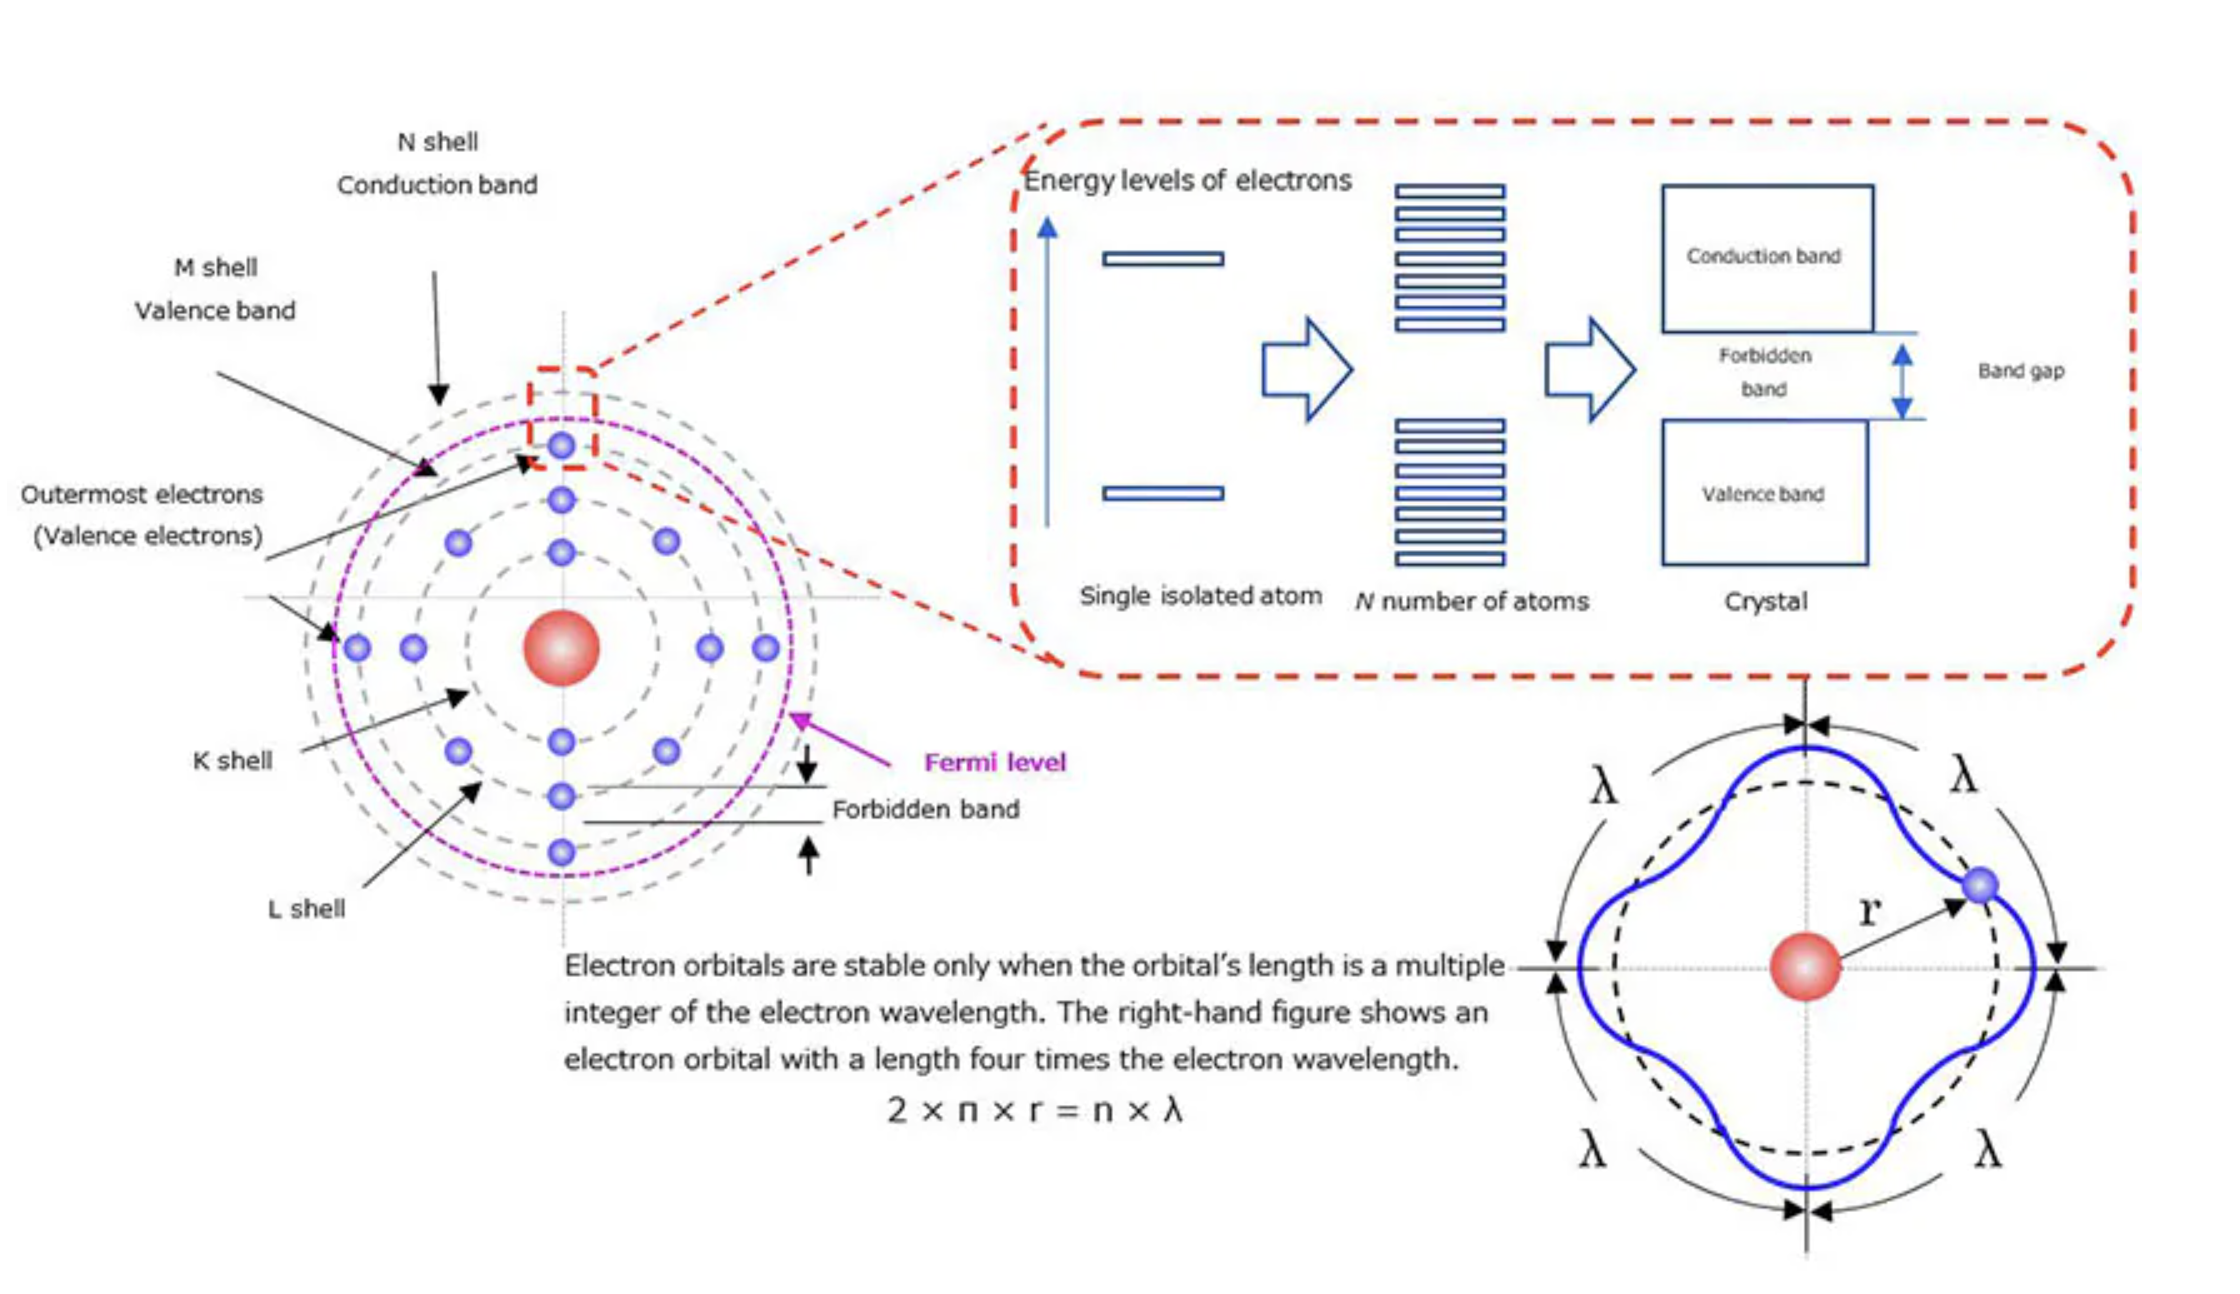
\includegraphics[width=\textwidth]{img/bohr_model_and_energy_bands.png}
		\end{center}
	\section{Positive Charges? Holes?}
		Now what's up with holes? 
	\section{How Does Doping Make Silicon Conductive?}
\end{document}